% Copyright 2004 by Till Tantau <tantau@users.sourceforge.net>.
%
% In principle, this file can be redistributed and/or modified under
% the terms of the GNU Public License, version 2.
%
% However, this file is supposed to be a template to be modified
% for your own needs. For this reason, if you use this file as a
% template and not specifically distribute it as part of a another
% package/program, I grant the extra permission to freely copy and
% modify this file as you see fit and even to delete this copyright
% notice. 

\documentclass{beamer}

% There are many different themes available for Beamer. A comprehensive
% list with examples is given here:
% http://deic.uab.es/~iblanes/beamer_gallery/index_by_theme.html
% You can uncomment the themes below if you would like to use a different
% one:
%\usetheme{AnnArbor}
%\usetheme{Antibes}
%\usetheme{Bergen}
%\usetheme{Berkeley}
%\usetheme{Berlin}
%\usetheme{Boadilla}
%\usetheme{boxes}
%\usetheme{CambridgeUS}
%\usetheme{Copenhagen}
%\usetheme{Darmstadt}
%\usetheme{default}
%\usetheme{Frankfurt}
%\usetheme{Goettingen}
%\usetheme{Hannover}
%\usetheme{Ilmenau}
%\usetheme{JuanLesPins}
%\usetheme{Luebeck}
\usetheme{Madrid}
%\usetheme{Malmoe}
%\usetheme{Marburg}
%\usetheme{Montpellier}
%\usetheme{PaloAlto}
%\usetheme{Pittsburgh}
%\usetheme{Rochester}
%\usetheme{Singapore}
%\usetheme{Szeged}
%\usetheme{Warsaw}

\title{Column Generation}

% A subtitle is optional and this may be deleted
\subtitle{}

\author{Renan S. Silva\inst{1}}
% - Give the names in the same order as the appear in the paper.
% - Use the \inst{?} command only if the authors have different
%   affiliation.

\institute[Udesc] % (optional, but mostly needed)
{
  \inst{1}%
  Computer Science Department\\
  Santa Catarina State University
}
% - Use the \inst command only if there are several affiliations.
% - Keep it simple, no one is interested in your street address.

%\date{Conference Name, 2013}
% - Either use conference name or its abbreviation.
% - Not really informative to the audience, more for people (including
%   yourself) who are reading the slides online

\subject{Theoretical Computer Science}
% This is only inserted into the PDF information catalog. Can be left
% out. 

% If you have a file called "university-logo-filename.xxx", where xxx
% is a graphic format that can be processed by latex or pdflatex,
% resp., then you can add a logo as follows:

% \pgfdeclareimage[height=0.5cm]{university-logo}{university-logo-filename}
% \logo{\pgfuseimage{university-logo}}

% Delete this, if you do not want the table of contents to pop up at
% the beginning of each subsection:
\AtBeginSubsection[]
{
  \begin{frame}<beamer>{Outline}
    \tableofcontents[currentsection,currentsubsection]
  \end{frame}
}

% Let's get started
\begin{document}

\begin{frame}
  \titlepage
\end{frame}

\begin{frame}{Outline}
  \tableofcontents
  % You might wish to add the option [pausesections]
\end{frame}

% Section and subsections will appear in the presentation overview
% and table of contents.
\section{What it is}  

\begin{frame}{What it is}
    Column Generation:
    
    \begin{itemize}
        \item Solves integer linear problems
        \item Manage the huge amount of variables
        \item Iteratively generate new columns
    \end{itemize}
\end{frame}

\begin{frame}{Rows Versus Columns}
    Huge amount of rows:
    
    \begin{minipage}{0.49\textwidth}
    $
     \begin{matrix}
      0         & 0 & 0      & 1 & 0 \\
      1         & 1 & 0      & 0 & 1 \\
      0         & 1 & 1      & 0 & 0 \\
         \vdots &   &        &   & \vdots \\
         \vdots &   &        &   & \vdots \\
      \vdots    &   & \ddots &   & \vdots \\
         \vdots &   &        &   & \vdots \\
         \vdots &   &        &   & \vdots \\
      0         & 1 & 1      & 0 & 0 \\
     \end{matrix}
    $
    \end{minipage}
    \begin{minipage}{0.49\textwidth}
    Examples
    \begin{itemize}
        \item TSP
    \end{itemize}
    \end{minipage}
\end{frame}


\begin{frame}{Rows Versus Columns}
    Huge amount of columns:

    \begin{minipage}{0.49\textwidth}
    $
     \begin{matrix}
      0 & 0 & \hdots & 1 & 0 \\
      0 & 1 &        & 0 & 1 \\
      1 & 0 & \ddots & 1 & 0 \\
      0 & 1 &        & 0 & 1 \\
      1 & 1 & \hdots & 1 & 1 \\
     \end{matrix}
    $
    \end{minipage}
    \begin{minipage}{0.49\textwidth}
    Examples
    \begin{itemize}
        \item Cutting Stock
        \item Crew Scheduling Problem
        \item Vehicle Routing Problem
    \end{itemize}
    \end{minipage}
\end{frame}

\section{Why should I use it}

\begin{frame}{Why should I use it}
    Motivation for using specialized methods:
    \begin{itemize}
        \item It is faster
        \item For a huge amount of rows, only a few have effect
        \item For a huge amount of columns, only a few are non zero
    \end{itemize}
\end{frame}

\section{How it works}

\begin{frame}{How it works}
    \begin{figure}
        \centering
        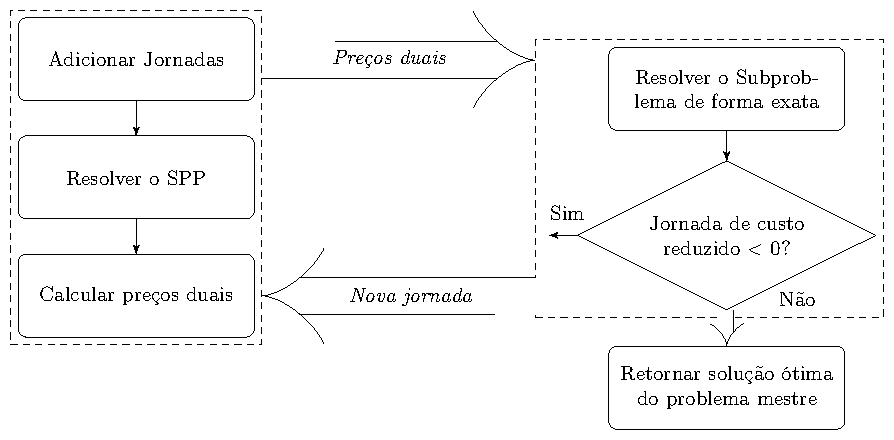
\includegraphics[width=0.9\textwidth]{gercolumn.pdf}
        \caption{How it works}
        \label{fig:my_label}
    \end{figure}
\end{frame}

\begin{frame}{Components}
    \begin{minipage}{0.49\textwidth}
    Reduced Master Problem (RMP)
    \begin{itemize}
        \item Contains a reduced set of columns from the original problem
        \item Solves the original problem
        \item Provides the (dual) info for the subproblem
    \end{itemize}
    \end{minipage}
    \begin{minipage}{0.49\textwidth}
    Subproblem
    \begin{itemize}
        \item Proves the optimality of the RMP
        \item Creates new columns (one at a time)
    \end{itemize}
    \end{minipage}
\end{frame}

\section{An Example}

\begin{frame}{Crew Scheduling Problem}
The Model:
   \begin{subequations}
    \begin{align}
        \text{Minimize:}\notag \\
        &\sum_{i,j} c_{ij} x_{ij} \\
        \text{Subject to:} \\
        &\sum_{k} x_{jk} = \sum_{i} x_{ij}, \text{ for }j = 1 \ldots N \\
        &\sum_{k} x_{jk} = 1, \text{ for }i = 1 \ldots N   \\
        &\sum_{j} x_{0j} = K   \\
        &\text{time limit constraints} \\
        &x_{ij} \in (0, 1) \forall i, j
    \end{align}
   \end{subequations}
\end{frame}

\begin{frame}{Crew Scheduling Problem}
The Other Model:
    \begin{figure}[!htb]
        \begin{minipage}{0.48\textwidth}
            \centering
                \begin{center}
                {
                \centering
                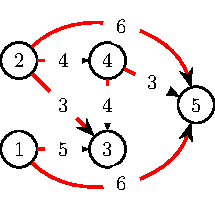
\includegraphics[width=0.8\textwidth]{graph.pdf}
                }
                \end{center}
        \end{minipage}
        \begin{minipage}{.48\textwidth}
            \begin{tabular}{l l l}
                Journey                           & Cost & Duration \\
                1 $\rightarrow$ 3                 & 5     & 13 \\
                1 $\rightarrow$ 5                 & 6     & 14 \\
                2 $\rightarrow$ 3                 & 3     & 13 \\
                2 $\rightarrow$ 4                 & 4     & 9  \\
                2 $\rightarrow$ 4 $\rightarrow$ 5 & 7     & 14 \\
                2 $\rightarrow$ 4 $\rightarrow$ 3 & 8     & 13 \\
                2 $\rightarrow$ 5                 & 6     & 14 \\
            \end{tabular}
        \end{minipage}
    \end{figure}
\end{frame}

\begin{frame}{Crew Scheduling Problem}
The Other Model:
    \begin{figure}[!htb]
        \centering
        \begin{minipage}{0.48\textwidth}
            $A = \begin{pmatrix}
                1 & 1 & 0 & 0 & 0 & 0 & 0 \\
                0 & 0 & 1 & 1 & 1 & 1 & 1 \\
                1 & 0 & 1 & 0 & 0 & 1 & 0 \\
                0 & 0 & 0 & 1 & 1 & 1 & 0 \\
                0 & 1 & 0 & 0 & 1 & 0 & 1 \\
            \end{pmatrix}$
        \end{minipage}
%
        \begin{minipage}{.48\textwidth}
            \begin{subequations}
                \label{spppp}
                \begin{align}
                \label{spp2}  \text{min} \: \sum_{j \in J} c_j x_j \\
                \label{spp22} \sum_{j \in J} a_{ij} x_j = 1, \forall i \in I \\
                \label{spp24} x_j \in \{0, 1\}, \forall j \in J
            \end{align}
        \end{subequations}
        \end{minipage}
    \end{figure}
\end{frame}

\begin{frame}{Reduced Master Problem}
    \begin{subequations}
        \label{pmaster}
        \begin{align}
            \label{pmaster1}  \text{min} \: &\sum_{j \in \tilde{J}} c_j x_j \\
            \label{pmaster2} &\sum_{j \in \tilde{J}} a_{tj} x_j = 1, \forall t \in T \\
            \label{pmaster3} &\sum_{j \in \tilde{J}}        x_j = NJ \\
            \label{pmaster4} x_j &\geq 0, \forall j \in \tilde{J}
        \end{align}
    \end{subequations}
\end{frame}

\begin{frame}{Subproblem}
    \begin{subequations}
        \label{subp}
        \begin{align}
            \label{subp1} \text{min} \: \sum_{a \in A} c_a y_a &- \sum_{t \in T} \tilde{\pi}_t v_t - \tilde{\mu}\\
            \label{subp2} \sum_{a \in \delta^{+} (v_0)} y_{a} &= \sum_{a \in \delta^{-} (v_f)} y_{a} = 1 \\
            \label{subp3} \sum_{a \in \delta^{+} (v_t)} y_{a} &= \sum_{a \in \delta^{-} (v_t)} y_{a} = v_t, \forall t \in T \\
            \label{subp4} \sum_{a \in A} d_a y_{a} &\leq MaxW \\
            \label{subp5} v_t, y_a &\in \{0, 1\}, \forall v_j \in V, \forall a \in A
        \end{align}
    \end{subequations}
\end{frame}

\begin{frame}{Crew Scheduling Problem}
    First Step
    \begin{figure}[!htb]
        %\begin{minipage}{0.48\textwidth}
            \centering
                %\begin{center}
                %{
                %\centering
                %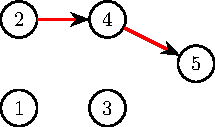
\includegraphics[width=0.8\textwidth]{graph2.pdf}
                %}
                %\end{center}
        %\end{minipage}
            $A = \begin{pmatrix}
                1 \\
                1 \\
                1 \\
                1 \\
                1 \\
            \end{pmatrix}$
    \end{figure}
\end{frame}

\begin{frame}{Crew Scheduling Problem}
    Second Step
    \begin{figure}[!htb]
        \begin{minipage}{0.48\textwidth}
            \centering
            $Y = \begin{pmatrix}56\\ 0\\ 0\\ 0\\ 0\\ -0\\ \end{pmatrix}$
            \end{minipage}
        \begin{minipage}{0.48\textwidth}
            $A = \begin{pmatrix}
                1 & 1 \\
                1 & 0 \\
                1 & 0 \\
                1 & 0 \\
                1 & 0 \\
            \end{pmatrix}$
        \end{minipage}
    \end{figure}
\end{frame}

\begin{frame}{Crew Scheduling Problem}
    Third Step
    \begin{figure}[!htb]
        \begin{minipage}{0.48\textwidth}
            \centering
            $Y = \begin{pmatrix}0\\ 56\\ 0\\ 0\\ 0\\ -0\\ \end{pmatrix}$
            \end{minipage}
        \begin{minipage}{0.48\textwidth}
            $A = \begin{pmatrix}
                1 & 1 & 0 \\
                1 & 0 & 1 \\
                1 & 0 & 0 \\
                1 & 0 & 0 \\
                1 & 0 & 0 \\
            \end{pmatrix}$
        \end{minipage}
    \end{figure}
\end{frame}

\begin{frame}{Crew Scheduling Problem}
    4th Step
    \begin{figure}[!htb]
        \begin{minipage}{0.48\textwidth}
            \centering
            $Y = \begin{pmatrix}0\\ 0\\ 56\\ 0\\ 0\\ -0\\ \end{pmatrix}$
            \end{minipage}
        \begin{minipage}{0.48\textwidth}
            $A = \begin{pmatrix}
                1 & 1 & 0 & 0 \\
                1 & 0 & 1 & 0 \\
                1 & 0 & 0 & 1 \\
                1 & 0 & 0 & 0 \\
                1 & 0 & 0 & 0 \\
            \end{pmatrix}$
        \end{minipage}
    \end{figure}
\end{frame}

\begin{frame}{Crew Scheduling Problem}
    5th Step
    \begin{figure}[!htb]
        \begin{minipage}{0.48\textwidth}
            \centering
            $Y = \begin{pmatrix}0\\ 0\\ 0\\ 56\\ 0\\ -0\\ \end{pmatrix}$
            \end{minipage}
        \begin{minipage}{0.48\textwidth}
            $A = \begin{pmatrix}
                1 & 1 & 0 & 0 & 0 \\
                1 & 0 & 1 & 0 & 0 \\
                1 & 0 & 0 & 1 & 0 \\
                1 & 0 & 0 & 0 & 1 \\
                1 & 0 & 0 & 0 & 0 \\
            \end{pmatrix}$
        \end{minipage}
    \end{figure}
\end{frame}

\begin{frame}{Crew Scheduling Problem}
    6th Step
    \begin{figure}[!htb]
        \begin{minipage}{0.48\textwidth}
            \centering
            $Y = \begin{pmatrix}0\\ 0\\ 0\\ 0\\ 56\\ -0\\ \end{pmatrix}$
            \end{minipage}
        \begin{minipage}{0.48\textwidth}
            $A = \begin{pmatrix}
                1 & 1 & 0 & 0 & 0 & 0\\
                1 & 0 & 1 & 0 & 0 & 0\\
                1 & 0 & 0 & 1 & 0 & 0\\
                1 & 0 & 0 & 0 & 1 & 0\\
                1 & 0 & 0 & 0 & 0 & 1\\
            \end{pmatrix}$
        \end{minipage}
    \end{figure}
\end{frame}

\begin{frame}{Crew Scheduling Problem}
    7th Step
    \begin{figure}[!htb]
        \begin{minipage}{0.48\textwidth}
            \centering
            $Y = \begin{pmatrix}14\\ 14\\ 14\\ 14\\ 14\\ -14\\ \end{pmatrix}$
                \begin{center}
                {
                \centering
                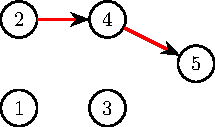
\includegraphics[width=0.5\textwidth]{graph2.pdf}
                }
                \end{center}
            \end{minipage}
        \begin{minipage}{0.48\textwidth}
            $A = \begin{pmatrix}
                1 & 1 & 0 & 0 & 0 & 0 & 1\\
                1 & 0 & 1 & 0 & 0 & 0 & 0\\
                1 & 0 & 0 & 1 & 0 & 0 & 1\\
                1 & 0 & 0 & 0 & 1 & 0 & 1\\
                1 & 0 & 0 & 0 & 0 & 1 & 0\\
            \end{pmatrix}$
        \end{minipage}
    \end{figure}
\end{frame}

\begin{frame}{Crew Scheduling Problem}
    8th Step
    \begin{figure}[!htb]
        \begin{minipage}{0.48\textwidth}
            \centering
            $Y = \begin{pmatrix}24.5\\ 24.5\\ 24.5\\ 24.5\\ -17.5\\ -24.5\\ \end{pmatrix}$
                \begin{center}
                {
                \centering
                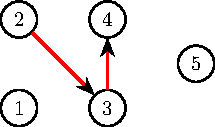
\includegraphics[width=0.5\textwidth]{graph3.pdf}
                }
                \end{center}
            \end{minipage}
        \begin{minipage}{0.48\textwidth}
            $A = \begin{pmatrix}
                1 & 1 & 0 & 0 & 0 & 0 & 0 & 0 \\
                1 & 0 & 1 & 0 & 0 & 0 & 1 & 1 \\
                1 & 0 & 0 & 1 & 0 & 0 & 0 & 1 \\
                1 & 0 & 0 & 0 & 1 & 0 & 1 & 1 \\
                1 & 0 & 0 & 0 & 0 & 1 & 1 & 0 \\
            \end{pmatrix}$
        \end{minipage}
    \end{figure}
\end{frame}

\begin{frame}{Crew Scheduling Problem}
    9th Step
    \begin{figure}[!htb]
        \begin{minipage}{0.48\textwidth}
            \centering
            $Y = \begin{pmatrix} 24.5\\ -16.5\\ 24.5\\ 24.5\\ 23.5\\ -24.5\\ \end{pmatrix}$
                \begin{center}
                {
                \centering
                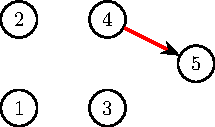
\includegraphics[width=0.5\textwidth]{graph4.pdf}
                }
                \end{center}
            \end{minipage}
        \begin{minipage}{0.48\textwidth}
            $A = \begin{pmatrix}
                \ldots & 0 & 0 & 0 \\
                \ldots & 1 & 1 & 0 \\
                \ldots & 0 & 1 & 0 \\
                \ldots & 1 & 1 & 1 \\
                \ldots & 1 & 0 & 1 \\
            \end{pmatrix}$
        \end{minipage}
    \end{figure}
\end{frame}


\begin{frame}{Crew Scheduling Problem}
    10th Step
    \begin{figure}[!htb]
        \begin{minipage}{0.48\textwidth}
            \centering
            $Y = \begin{pmatrix} 24.5\\ 4\\ 24.5\\ 4\\ 23.5\\ -24.5\\ \end{pmatrix}$
                \begin{center}
                {
                \centering
                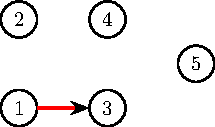
\includegraphics[width=0.5\textwidth]{graph5.pdf}
                }
                \end{center}
            \end{minipage}
        \begin{minipage}{0.48\textwidth}
            $A = \begin{pmatrix}
                \ldots & 0 & 0 & 0 & 1 \\
                \ldots & 1 & 1 & 0 & 0 \\
                \ldots & 0 & 1 & 0 & 1 \\
                \ldots & 1 & 1 & 1 & 0 \\
                \ldots & 1 & 0 & 1 & 0 \\
            \end{pmatrix}$
        \end{minipage}
    \end{figure}
\end{frame}

\begin{frame}{Crew Scheduling Problem}
    11th Step
    \begin{figure}[!htb]
        \begin{minipage}{0.48\textwidth}
            \centering
            $Y = \begin{pmatrix} 5\\ 4\\ 5\\ 4\\ 4\\ -5\\ \end{pmatrix}$
                \begin{center}
                {
                \centering
                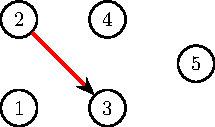
\includegraphics[width=0.5\textwidth]{graph6.pdf}
                }
                \end{center}
            \end{minipage}
        \begin{minipage}{0.48\textwidth}
            $A = \begin{pmatrix}
                \ldots & 0 & 0 & 0 & 1 & 0 \\
                \ldots & 1 & 1 & 0 & 0 & 1 \\
                \ldots & 0 & 1 & 0 & 1 & 1 \\
                \ldots & 1 & 1 & 1 & 0 & 0 \\
                \ldots & 1 & 0 & 1 & 0 & 0 \\
            \end{pmatrix}$
        \end{minipage}
    \end{figure}
\end{frame}


\begin{frame}{Crew Scheduling Problem}
    12th Step
    \begin{figure}[!htb]
        \begin{minipage}{0.48\textwidth}
            \centering
            $Y = \begin{pmatrix} 6\\ 4\\ 5\\ 5\\ 4\\ -6\\ \end{pmatrix}$
                Reduced cost $=$ $0$
            \end{minipage}
        \begin{minipage}{0.48\textwidth}
            $A = \begin{pmatrix}
                \ldots & 0 & 0 & 0 & 1 & 0 \\
                \ldots & 1 & 1 & 0 & 0 & 1 \\
                \ldots & 0 & 1 & 0 & 1 & 1 \\
                \ldots & 1 & 1 & 1 & 0 & 0 \\
                \ldots & 1 & 0 & 1 & 0 & 0 \\
            \end{pmatrix}$
        \end{minipage}
    \end{figure}
\end{frame}

\begin{frame}{Crew Scheduling Problem}
    Solution
    %{
        %$\begin{matrix}
            %1 & 1 & 0 & 0 & 0 & 0 & 0 & 0 & 0 & 0 & 1 & 0 \\
            %1 & 0 & 1 & 0 & 0 & 0 & 1 & 1 & 1 & 0 & 0 & 1 \\
            %1 & 0 & 0 & 1 & 0 & 0 & 0 & 1 & 1 & 0 & 1 & 1 \\
            %1 & 0 & 0 & 0 & 1 & 0 & 1 & 1 & 1 & 1 & 0 & 0 \\
            %1 & 0 & 0 & 0 & 0 & 1 & 1 & 0 & 0 & 1 & 0 & 0 \\
        %\end{matrix}$
    %}

        \begin{center}
        {
        \centering
        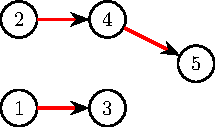
\includegraphics[width=0.5\textwidth]{graph666.pdf}
        }
        \end{center}
\end{frame}

\end{document}


